\chapter{Unmodified band structure}
The linear electronic dispersion of graphene was published by Wallace\cite{Wallace1947} 57 years before Geim, Novoselov and co-workers spurred graphene research forward with their method of mechanical exfoliation\cite{Novoselov2004}.
In 1984 Semenoff formalized the equivalence between the low energy electrons in graphene and Dirac-Weyl electrons \cite{Semenoff1984}.
Remarkably, the nearest neighbor tight binding approach used by these authors has accurately described the majority of the low energy physics in graphene.
This chapter will follow in the spirit of these derivations but give additional emphasis to prepare for the discussion of the strain induced pseudo vector potential and the phonon induced Kekul\'e transition.

\section{Graphene's lattice and Brillouin zone}
\begin{figure}
	\begin{center}
	% Geometry taken directly from pg 1 of little moleskin theory book
\newcommand{\alat}{1 cm}
\newcommand{\sqth}{1.73205080757}
\newcommand{\Klen}{2 cm}
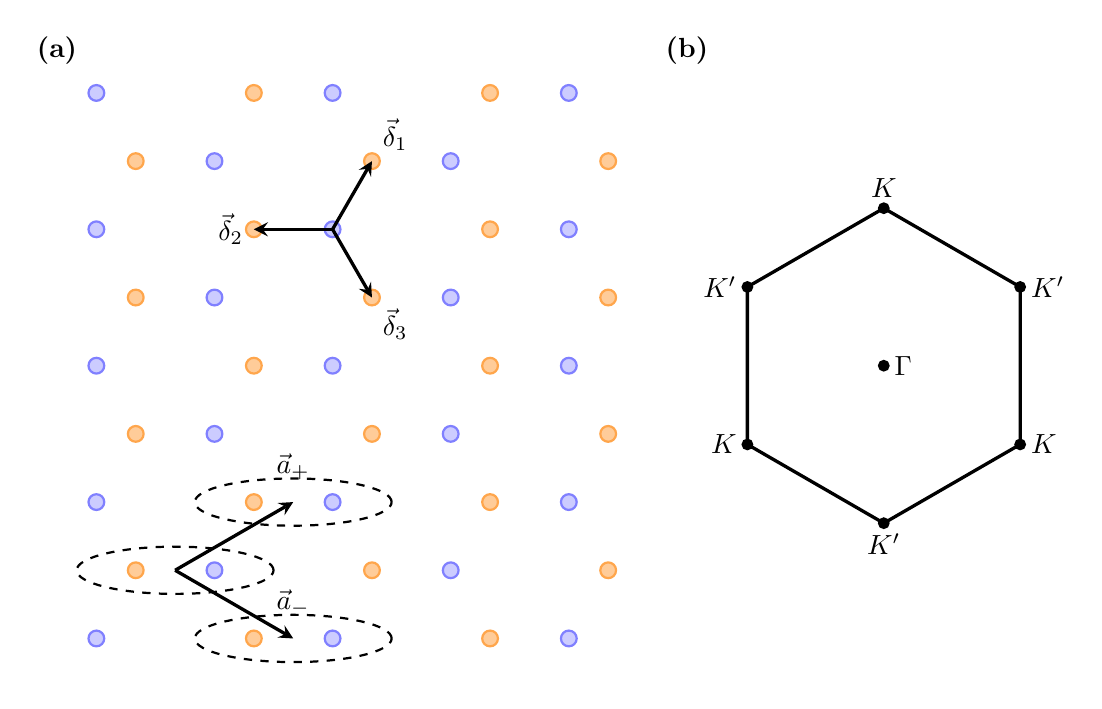
\begin{tikzpicture}															

	% Graphene lattice, sublattices different colors, nearest neighbor vectors and lattice vectors
	\begin{scope}[xshift=-3.5 cm,>=stealth,
		nnarrow/.style={color=black,very thick, ->},					% Nearest neighbor vectors
		A/.style={circle,draw=blue!50,fill=blue!20,
			thick,minimum size=2 mm,inner sep=0pt}, 					% A sublattice dots
		B/.style={circle,draw=orange!70,fill=orange!40,
			thick,minimum size=2mm,inner sep=0pt},						% B sublattice dots
		el1/.style={x radius=1.25*\alat,y radius=.3*\alat},				% Style for the ellipse
		el2/.style={dashed,thick}]										% Style for the ellipse draw

		%This scope is clipped to limit the drawn lattice to a square
		\clip (-3.5cm,-4cm) rectangle(4cm,4cm);
		% Draw the lattice
		\foreach \ip in {-3,-2,...,3}
			\foreach \im in {-3,-2,...,3}
			{
			\node at (\ip*\alat*3/2+\im*\alat*3/2      ,\ip*\sqth*\alat/2-\im*\sqth*\alat/2) [A] {};
			\node at (\ip*\alat*3/2+\im*\alat*3/2-\alat,\ip*\sqth*\alat/2-\im*\sqth*\alat/2) [B] {};
			}

		% Draw the nearest neighbor vectors
		\draw[nnarrow] (0,\alat*\sqth) -- +(60 :\alat) node[anchor=south west]{$\vec{\delta}_1$};
		\draw[nnarrow] (0,\alat*\sqth) -- +(180:\alat) node[anchor=east      ]{$\vec{\delta}_2$};
		\draw[nnarrow] (0,\alat*\sqth) -- +(-60:\alat) node[anchor=north west]{$\vec{\delta}_3$};
		
		% Draw the lattice vectors
		\draw[nnarrow] (240:3*\alat) ++(-\alat/2,0) -- +( 30:\sqth*\alat) node[circle,anchor=south]{$\vec{a}_+$};
		\draw[nnarrow] (240:3*\alat) ++(-\alat/2,0) -- +(-30:\sqth*\alat) node[circle,anchor=south]{$\vec{a}_-$};

		% Ellipses around two atom basis
		\draw[el2] (240:3*\alat) ++(-\alat/2,0) +(  0,0          ) ellipse[el1];
		\draw[el2] (240:3*\alat) ++(-\alat/2,0) +( 30:\sqth*\alat) ellipse[el1];
		\draw[el2] (240:3*\alat) ++(-\alat/2,0) +(-30:\sqth*\alat) ellipse[el1];
	\end{scope}

	% Reciprocal space BZ and high symmetry points
	\begin{scope}[xshift=3.5cm,
		BZ/.style={color=black,fill=black,very thick},
		circ2/.style={radius=1.5pt}]

		% Draw the BZ
		\draw[BZ]
			( 30:\Klen) circle[circ2] node[anchor=west] {$\bm{K'}$} --
			( 90:\Klen) circle[circ2] node[anchor=south]{$\bm{K}$}  --
			(150:\Klen) circle[circ2] node[anchor=east] {$\bm{K'}$} -- 
			(210:\Klen) circle[circ2] node[anchor=east] {$\bm{K}$}  -- 
			(270:\Klen) circle[circ2] node[anchor=north]{$\bm{K'}$} -- 
			(330:\Klen) circle[circ2] node[anchor=west] {$\bm{K}$}  -- 
			( 30:\Klen);

		% Label the high symmetry points
		\draw[BZ] (0,0) circle[circ2] node[anchor=west]{$\Gamma$};
	\end{scope}

	% (a) and (b) labels
	\node at (-7cm,4cm) {\textbf{(a)}};
	\node at ( 1cm,4cm) {\textbf{(b)}};
\end{tikzpicture}
	\end{center}
	\caption{\label{fig:TB:geometry} (a) Real space graphene lattice with the A sub-lattice in orange, the B sub-lattice in blue, nearest neighbor vectors ($\vec \delta_1$, $\vec \delta_2$, and $\vec \delta_3$) shown as arrows, and lattice vectors ($\vec a_+$ and $\vec a_-$) shown translating the two atom basis. (b) First Brillouin zone with the $\Gamma$ point and equivalent $\bm{K}$ and $\bm{K'}$ points indicated.}
\end{figure}

In its unperturbed state, the carbon atoms in the graphene lattice are arrayed in a hexagon as shown in Figure \ref{fig:TB:geometry}(a).
Throughout the x axis will be taken in the zigzag direction as shown.
Since a hexagonal lattice is not a Bravais lattice, the lattice is treated as a triangular Bravais lattice with a two atom bases.
In figure \ref{fig:TB:geometry}(a) the A sub-lattice is colored orange and the B sub-lattice is colored blue.
The lattice is created by arraying the two atoms basic using the lattice vectors 
\begin{align*}
	\vec{a}_+&= \frac{\sqrt{3}a}{2} \hat{x} + \frac{3a}{2} \hat{y} \\
	\vec{a}_-&=-\frac{\sqrt{3}a}{2} \hat{x} + \frac{3a}{2} \hat{y}
\end{align*}
where $a=1.4 \ l\angstrom$ is the nearest neighbor distance.
The three nearest neighbor vectors are given by:
\begin{align*}
	\vec \delta_1&=-\frac{\sqrt{3} a}{2}\hat{x}+\frac{a}{2}\hat{y}\\
	\vec \delta_2&= \frac{\sqrt{3} a}{2}\hat{x}+\frac{a}{2}\hat{y}\\
	\vec \delta_3&=a \hat{y}
\end{align*}

The Brillouin zone of graphene is shown in Figure \ref{fig:TB:geometry}(b).
Like the graphene lattice the Brillouin zone is hexagonal, however it is rotated 30 degrees relative to the crystal axis.
The $\Gamma$ point is at the center of the Brillouin zone while the $\bm{K}$ and $\bm{K'}$ are at the corners.
It should be noted that only 2 of the 6 corners of the hexagon are unique, the others can be connected by reciprocal lattice vectors.
The position of the $\bm{K}$ and $\bm{K'}$ points are given by:
\begin{align*}
	\bm{K}&=-\bm{K'}= \frac{4 \pi}{3 \sqrt{3} a} \hat{x} \\
	\bm{K}&=-\bm{K'}=-\frac{2 \pi}{3 \sqrt{3} a} \hat{x} + \frac{2 \pi}{3 a} \hat{y} \\
	\bm{K}&=-\bm{K'}=-\frac{2 \pi}{3 \sqrt{3} a} \hat{x} - \frac{2 \pi}{3 a} \hat{y},
\end{align*}
with the first pair the easiest to work with.

In later sections this discussion will be expanded to take into account strain and phonons perturbing the graphene lattice.
In both cases the changes in graphene's electronic dispersion originates from changes in the position of the atoms.

\section{Electronic dispersion}
Since the tight binding formalism is used universally in this work, this section will start with a brief motivation of its form.
Afterward, the nearest neighbor tight binding formalism will be applied to graphene.

In second quantization, the total energy in the system is written as:
\begin{equation*}
	H=\sum_{\vec{k},\sigma} c^{\dagger}_{\vec{k},\sigma} c_{\vec{k},\sigma} \epsilon_{\vec{k}}
\end{equation*}
where $c^{\dagger}_{\vec{k},\sigma}$ and $c_{\vec{k},\sigma}$ are the creation and annihilation operators for an electrons with wave-vector $\vec{k}$ and spin $\sigma$ and $\epsilon_{\vec{k}}$ is the energy of the electron with wave-vector $\vec{k}$.
The product $c^{\dagger}_{\vec{k},\sigma} c_{\vec{k},\sigma}$ is then a number operator.
This is a very natural definition of the energy; the equation simply sums the energy one wave-vector at a time.

% Here justification of this approximation--applicable when atoms aren't too close...
\begin{align*}
	c^{\dagger}_{\vec{k},\sigma}&=\frac{1}{\sqrt{N}}\sum_{\vec{R}_i} e^{ i \vec{k} \cdot \vec{R}_i} c_{i,\sigma} \\
	c          _{\vec{k},\sigma}&=\frac{1}{\sqrt{N}}\sum_{\vec{R}_i} e^{-i \vec{k} \cdot \vec{R}_i} c_{i,\sigma} \\
\end{align*}
The Hamiltonian becomes:
\begin{align*}
	H&=-\sum_{\vec{R}_i, \vec{R}_j,\sigma} (-) \sum_{\vec{k}}\frac{1}{N} e^{i \vec{k} \cdot (\vec{R}_i-\vec{R}_j)}
	 \epsilon_{\vec{k}} c^{\dagger}_{i,\sigma} c_{j,\sigma} \\
	 &=-\sum_{<i,j>,\sigma} t_{i,j} c^{\dagger}_{i,\sigma} c_{j,\sigma} + \text{H.C},\\
\end{align*}
where the final sum is over $<i,j>$ nearest neighbor pairs and $t_{i,j}=-\sum_{\vec{k}}\frac{1}{N} e^{i \vec{k} \cdot (\vec{R}_i-\vec{R}_j)}\epsilon_{\vec{k}}$ is the hopping energy.
This seemingly complicated parameter has an easy interpretation when the final form of the Hamiltonian is considered.
The hopping energy is the energy associated with removing an electron from atom $j$ and putting it on atom $i$.
As will be illustrate for graphene, this tight binding formalism provides a simple but powerful method of calculating band structures.

The physics relevant for this work is captured by the nearest neighbor tight binding model, the lowest order tight binding approximation.
For graphene, when an electron hops between nearest neighbor, it changes sub-lattice.
The nearest neighbor Hamiltonian reflects this:
\begin{equation*}
	H=-t \sum_{<i,j>} (a_i^{\dagger} b_j + \text{H.C.}),
\end{equation*}
where the hopping energy $t$ gives the energy it takes to remove an electron from the jth atom in the B sub-lattice with the B sub-lattice annihilation operator $b_j$ and put an electron on it nearest neighbor, the ith atom in the A sub-lattice, using the A sub-lattice creation operator $a_i$.
The sum is restricted to $<i,j>$ nearest neighbor pairs.
Finally the Hermitian conjugate, $\text{H.C.}$, accounts for the hopping from the A sub-lattice to the B sub-lattice and also ensures that the Hamiltonian is Hermitian.

The Hamiltonian is simplified by writing the creation and annihilation operators in Fourier space.
There is some freedom in choosing the phase factors.
They can either be chosen so that the operators are expanded around the position of each atom or instead they can be expanded around the position of the atomic basis occupied by the atom.
Both approaches yield the same result if one is consistent\cite{Bena2009}.
Here the operators are expanded about the atomic basis.
This will make the correspondence with the Dirac-Weyl equation more clear.
\begin{align*}
	a_i^{\dagger}&=\frac{1}{\sqrt{N}}\sum_{\vec{k} } e^{ i \vec{k}  \cdot \vec{R}_i} a_{\vec{k} }^{\dagger} \\
	b_j          &=\frac{1}{\sqrt{N}}\sum_{\vec{k}'} e^{-i \vec{k}' \cdot \vec{R}_j} b_{\vec{k}'} \\
\end{align*}
where $R_i$ and $R_j$ are the position of the $ith$ and $jth$ atomic basis respectfully.  
Since we are limited to nearest neighbor pairs $R_j$ is restricted to $\vec{R}_j \in \{ \vec{R}_i,\vec{R}_i+\vec{a}_+,\vec{R}_i+\vec{a}_-\}$.
This is equivalent to saying the nearest neighbor is either in the same atomic basis or in one of the neighboring atomic basis. 
The Hamiltonian can now be written in Fourier space as
\begin{align}
	H&=-t \frac{1}{N} \sum_{\vec{k},\vec{k'}}\sum_i \left( e^{i \vec{R}_i \cdot (\vec{k}-\vec{k}')}
		\left( 1+e^{-i \vec{k}' \cdot \vec{a}_+}+e^{-i \vec{k}' \cdot \vec{a}_-} \right) 
		a^{\dagger}_{\vec{k}} b_{\vec{k}'} + \text{H.C.} \right)\\
	 &=-t \frac{1}{N} \sum_{\vec{k},\vec{k'}}\left( N \delta_{\vec{k},\vec{k'}}
	 	\left( 1+e^{-i \vec{k}' \cdot \vec{a}_+}+e^{-i \vec{k}' \cdot \vec{a}_-}\right) 
		a^{\dagger}_{\vec{k}} b_{\vec{k}'} + \text{H.C.}\right)\\ 
	 &=-t \sum_{\vec{k}}\left( h(\vec{k})a^{\dagger}_{\vec{k}} b_{\vec{k}} + \text{H.C.} \right)\\ 
\end{align}
or
\begin{equation}
	H=\sum_{\vec k} 
		\left( \begin{array}{cc} a^{\dagger}_{\vec{k}} & b^{\dagger}_{\vec{k}} \end{array} \right)
		\left( \begin{array}{cc}
			0              & -t h(\vec{k}) \\
			-t h*(\vec{k}) & 0                                                 \end{array} \right)
		\left( \begin{array}{c } a_{\vec{k}}           \\ b_{\vec{k}}          \end{array} \right) 
	\label{eq:TB:RealSpace}
\end{equation},
where,
\begin{equation}
	h(\vec{k})=1+e^{-i \vec{k} \cdot \vec{a}_+}+e^{-i \vec{k} \cdot \vec{a}_-}
		=1+2 e^{-i \frac{3}{2} k_y}\cos \left(\frac{\sqrt{3}}{2} a k_x \right)
	\label{eq:TB:hk}
\end{equation}
A straightforward calculation provides the full electrical dispersion,
\begin{equation*}
	E(\vec{k})=\pm t |h(\vec{k})|=\sqrt{1+4 \cos^2 \left(\frac{\sqrt{3}}{2} a k_x\right)
		+4 \cos\left(\frac{\sqrt{3}}{2} a k_x \right) \cos \left(\frac{3}{2} a k_y\right)},
\end{equation*}
which is plotted in figure \ref{fig:TB:Dispersion}.
As shown, the two energy bands converge at the corners of the Brillouin zone, meeting at single points.
When no extra charge carriers have been added through capacitive coupling or by charge transfer from contaminates, the Fermi energy sits at these points, with the lower energy band filled and the higher energy band empty. %Have to fill in why here
Thus, the low energy excitations happen about these points.
The nearest neighbor tight binding approach is fairly accurate in the low energy regime.
If information further from these points is needed, a higher order approximation is required to account for things such as triginol warping.

\begin{figure}
	\begin{center}
	\begin{tikzpicture}[>=stealth,scale=.8,
	setts/.style={color=black,very thick, ->},
	cross/.style={color=black,very thick}]

	\node at (0,0) {\includegraphics{Figs_TightBinding/bandstructure_thesis.png}};
	\node at (-5,0)[anchor=center]{$\bm{K}$};
	\node at ( 5,0)[anchor=center]{$\bm{K'}$};

	% Coordinate axis
	\begin{scope}[xshift=-6cm,yshift=-6cm]
		\draw[setts] (0,0) -- (0,12 cm) node [anchor=south east] {$E$};
		\draw[setts] (0,0) -- (12 cm,0) node [anchor=north west] {$k_x$};
		% The out of plane axis
		\draw[cross] (-3 pt, -3 pt) -- ( 3 pt, 3 pt);
		\draw[cross] (-3 pt,  3 pt) -- ( 3 pt,-3 pt);
		\node at (0,0)[anchor=north east] {$k_y$};
		% \draw[fill=black,color=black] (0,0) circle[radius=3pt] node[anchor=north east] {$k_y$};
	\end{scope}
\end{tikzpicture}
	\end{center}
	\caption{\label{fig:TB:Dispersion} The electronic dispersion calculated with a nearest neighbor tight binding approach in the first Brillouin zone.  The two band meet at the $\bm{K}$ and $\bm{K'}$ points.}	
\end{figure}

The two points of convergence between the high and low energy bands are referred to as the Dirac points because of the characteristic energy dispersion near these points.
This interesting low energy physics can be best captured by expanding the Hamiltonian in equation \ref{eq:TB:RealSpace} about these points.
The wave-vectors near these points can be expressed as $\vec{k}=\bm{K}+\vec{q}$ and $\vec{k}=\bm{K'}+\vec{q}'$.
Expanding the $\vec{k}$ dependent term in the Hamiltonian for small $\vec{q}$ yields different values at the $\bm{K}$ and $\bm{K'}$ points.
\begin{align*}
	h(\bm{K }+\vec{q})&= -\frac{3}{2} a \left( q_x-i q_y \right) \\
	h(\bm{K'}+\vec{q}')&= -\frac{3}{2} a \left(-q_x-i q_y \right) . \\
\end{align*}
These values are independent of which of the three identical $\bm{K}$ or $\bm{K'}$ points are expanded about.
The Hamiltonian can now be expressed in the simpler form \ref{eq:TB:RealSpace}
\begin{align*}
	\bm{K:} \ H&=\frac{3}{2} a t \sum_{\vec q} 
		\left( \begin{array}{cc} a^{\dagger}_{\vec{q}} & b^{\dagger}_{\vec{q}} \end{array} \right)
		\left( \begin{array}{cc}
			0              & q_x - i q_y\\
			q_x+i q_y      & 0                                                 \end{array} \right)
		\left( \begin{array}{c } a_{\vec{q}}           \\ b_{\vec{q}}          \end{array} \right) \\
	  &=\frac{3}{2} a t \sum_{\vec q}
		\left( \begin{array}{cc} a^{\dagger}_{\vec{q}} & b^{\dagger}_{\vec{q}} \end{array} \right)
		\vec{q} \cdot \vec{\sigma}
		\left( \begin{array}{c } a_{\vec{q}}           \\ b_{\vec{q}}          \end{array} \right) \\
	\bm{K':} \ H&=\frac{3}{2} a t \sum_{\vec q'} 
		\left( \begin{array}{cc} b^{\dagger}_{\vec{q}'} & a^{\dagger}_{\vec{q}'} \end{array} \right)
		\left( \begin{array}{cc}
			0              & -q'_x + i q'_y\\
			-q'_x-i q'_y     & 0                                                 \end{array} \right)
		\left( \begin{array}{c } b_{\vec{q}'}           \\ a_{\vec{q}'}          \end{array} \right) \\
	  =&\frac{3}{2} a t \sum_{\vec q'}
		\left( \begin{array}{cc} b^{\dagger}_{\vec{q}'} & a^{\dagger}_{\vec{q}'} \end{array} \right)
		(-1)\vec{q}' \cdot \vec{\sigma}
		\left( \begin{array}{c } b_{\vec{q}'}           \\ a_{\vec{q}'}          \end{array} \right), \\
\end{align*}
or in the combined form:
\begin{align}
	H&=\frac{3}{2} a t \sum_{\vec q, \vec{q}'}
		\left( \begin{array}{cccc} b^{\dagger}_{\vec{q}} & a^{\dagger}_{\vec{q}} & a^{\dagger}_{\vec{q}'} & b^{\dagger}_{\vec{q}'}
																							\end{array} \right)
		\left( \begin{array}{cccc}
			0              & q_x - i q_y & 0            & 0 \\
			q_x+i q_y      & 0           & 0            & 0 \\                            
			0              & 0           & 0            & -q'_x+i q'_y \\
			0              & 0           & -q'_x-i q'_y & 0			            			\end{array} \right)
		\left( \begin{array}{c } b_{\vec{q}} \\ a_{\vec{q}} \\ a_{\vec{q}'} \\ b_{\vec{q}'}  \end{array} \right) \\
	H&=\sum_{\vec q, \vec{q}'}
		\left( \begin{array}{cccc}  a^{\dagger}_{\vec{q}} & b^{\dagger}_{\vec{q}}&  b^{\dagger}_{\vec{q}'} & a^{\dagger}_{\vec{q}'}
																							\end{array} \right)
		\left( \begin{array}{cc}
			v_f \vec{p} \cdot \vec{sigma}              & q_x - i q_y\\
			0              & v_f \vec{p'} \cdot \vec{sigma}			   	            			\end{array} \right)
		\left( \begin{array}{c }  a_{\vec{q}} \\ b_{\vec{q}} \\  b_{\vec{q}'} \\ a_{\vec{q}'} \end{array} \right)
	\label{eq:TB:FullH}
\end{align}
with $\vec{\sigma}= \left( \begin{array}{cc} 0 & 1 \\ 1 & 0 \end{array} \right) \hat{x}+\left( \begin{array}{cc} 0 & -i \\ i & 0 \end{array} \right) \hat{y}$ is the vector of Pauli matrices.
To express the Hamiltonian near the $\bm{K'}$ point in terms of Pauli matrices, the order of the raising and lower operators was switched.
This subtle difference means that the first component of eigenvectors corresponds to the amplitude for an electron on the B sublattice.
These approximate Hamiltonians will be central for the discussion of electron physics in manipulated graphene.

The eigenvalues near either $\bm{K}$ or $\bm{K'}$ are easy to solve for using the low energy Hamiltonians.
At both points, the low energy electronic dispersion is identical,
\begin{equation*}
	E=\pm \frac{3}{2}a t |\vec{q}|=\hbar v_f |\vec{q}| \ .
\end{equation*}
where $v_f$ is the Fermi velocity given by $\frac{3}{2}\frac{at}{\hbar} \sim .9 \times 10^6 \ m/s$.
As shown in Figure \ref{fig:TB:Dispersion}, the high and low energy bands meat at points at the Dirac points.
Away from this point, the energy scales linearly with momentum measured from the Dirac point.
Reminiscent of the light cone, this canonical dispersion is characteristic of a massless particle.

From the low energy electronic dispersion the density of electronic states can be directly calculated for the two dimensional system.
After taking account of the two full spin and two fold valley degeneracy, the density of states is:
\begin{equation}
	\rho(\epsilon)=\frac{2}{\pi} \left( \frac{\hbar v_f}{L} \right)^2 \epsilon
\end{equation}
where $L^2$ is the area of the graphene.
The linearity is due to the canonical energy dispersion.
The number of states at a given energy is just the circumference of the Dirac cone at this energy.
Using the density of states the chemical potential can be calculated in standard graphene transport experiments.

Graphene's two dimensional nature makes it simple to continuously modify the chemical potential.
Rather than varying the concentration of dopants as must be done for most three dimensional systems, graphene only requires the application of a back gate voltage.
A standard graphene gated device is shown in Figure \ref{fig:TB:FET}.
Changing the back gate voltage ($V_{BG}$) charges the graphene-backgate capacitor, introducing charges into the system.
In general, the differential increase in the number of charges is $dQ=C(\mu) dV$.
The capacitance is defined as:
\begin{equation}
	C=\frac{d N}{d \mu}
\end{equation}
where $N$ is the number of electrons in the graphene and $\mu$ is the chemical potential.
For intrinsic graphene the capacitance is continuous and the total number of charges is just $N=CV/e$.
The gated graphene device shown in Figure \ref{fig:TB:FET} can be treated as a parallel plate capacitor with a plate separation of 285 nm and the dielectric constant of silicon dioxide.
Matching the integrated density of states to the number of charges in the system relates the applied gate voltage to different measurements of the chemical potential in the system.
Some useful relationships are:
\begin{align*}
	n(cm^{-2})&\sim 7 \times 10^{10} V_{BG} (Volts) \\
	\mu(meV) &\sim 30 \sqrt{V_{BG} (Volts)} \\
	\mu(meV) &\sim 1 \times 10^{-7} \sqrt{n(cm^{-2})}
\end{align*}

\begin{figure}
	\begin{center}
	\newcommand{\FEThw}{4 cm}			% Width--1 cm=1 um
\newcommand{\FETsiot}{.3 cm}		% SiO2 thickness
\newcommand{\FETsit}{.7 cm}			% Si thickness
\newcommand{\FETaut}{0.06 cm}		% Au thickness
\newcommand{\FETauw}{2 cm}			% Separation and width of the gold pad
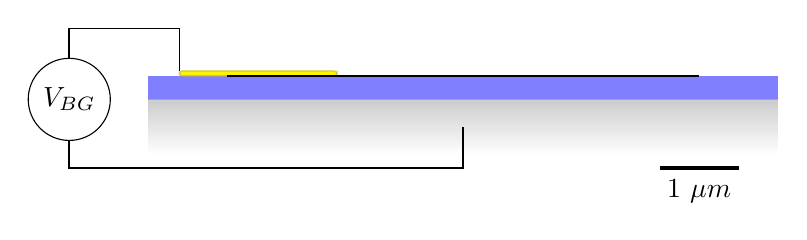
\begin{tikzpicture}[scale=1,
	sio2/.style={fill=blue!50!white,draw=none},
	si/.style={top color=black!20!white, bottom color=white},
	siedge/.style={draw=black!35!white},
	au/.style={fill=yellow,draw=black!20!yellow,rounded corners=1 pt},
	wire/.style={semithick}]
	
	%The SiO2
	\filldraw[sio2] (-\FEThw,0) rectangle (\FEThw,\FETsiot);

	%The Si
	\shade[si] (-\FEThw,-\FETsit) rectangle (\FEThw,0);
	\draw[siedge] (-\FEThw,0) -- (\FEThw,0);

	%The Gold contacts
	\filldraw[au] (-\FEThw*.9,\FETsiot) rectangle +(\FETauw,\FETaut);
	
	%The Graphene on the top
	\draw[semithick] (-3*\FEThw/4,\FETsiot) -- (3*\FEThw/4,\FETsiot);

	%The wires connecting the gate etc.
	\node (VBG) at (-1.25*\FEThw,0) [circle,draw=black]{$V_{BG}$};
	\draw[wire]  (VBG.north) -- (-1.25*\FEThw,2.5*\FETsiot+2.5*\FETaut) -- (-\FEThw*.9,2.5*\FETsiot+2.5*\FETaut) -- (-\FEThw*.	9,\FETsiot+\FETaut);
	\draw[wire]  (VBG.south) -- (-1.25*\FEThw,-1.25*\FETsit) -- (0,-1.25*\FETsit) -- (0,-.5*\FETsit);

	%Scale bar
	\draw[draw=black,ultra thick,xshift=.75*\FEThw, yshift=-\FETsit*1.25] (-.5 cm,0) -- node[anchor=north] {$1 \ \mu m$}(.5 cm, 0);

\end{tikzpicture}
	\end{center}
	\caption{\label{fig:TB:FET} Side view of a back gated graphene device.  The graphene is on top of 300 nm of thermal oxide grown on heavily doped Si. }	
\end{figure}

\section{Dirac-Weyl electrons}
Graphene's linear electrical dispersion is peculiar.
According to the usual expression for the effective mass of an electron in an electric field, $m^*=\frac{\hbar^2}{\frac{d^2 E}{d k^2}}$, \cite{Kittel2005} the electrons in graphene have infinite mass.
In a classical sense, this is understandable.
The electron's group velocity, $d \omega/d k$ is constant; it can not be changed by applying a force.
Classically, this corresponds to the case of an infinite mass which cannot be accelerated.
An alternative, and more enlightening, interpretation of graphene's properties is as a massless, relativistic, spin 1/2, fermion.
In this scenario the group velocity cannot be changed because the electrons are moving at the systems effective light speed.
Hence, like a photon moving at the speed of light graphene's electrons cannot be accelerated.

In 1984 Semenoff demonstrated that there is an exact correspondence between the low energy Hamiltonian of graphene and the two dimensional Dirac-Weyl Hamiltonian\cite{Semenoff1984} which governs massless, relativistic, spin 1/2, Fermions.
As a result, many phenomena from high energy physics have been observed in graphene including...
In this section this correspondence will be briefly discussed.

The Hamiltonian of general, relativistic, spin 1/2, fermions is known as the Dirac equation.
It is a matrix equation which is covariant, obeys the relativistic energy expression, and is first order in time.
For the special case of massless particles, the expression is simplified and, in a wisely chosen representation, is written as:
\begin{equation*}
	H=\left( \begin{array}{cc}
			c \vec{p} \cdot \vec{sigma}              & q_x - i q_y\\
			0              & c \vec{p} \cdot \vec{sigma}			   	            			\end{array} \right)
\end{equation*}
which, for particles in two spatial dimensions, is identical to Equation \ref{eq:TB:FullH}.
It is clear now that the electrons in graphene behave like relativistic particles in a system where the speed of light is given by the fermi velocity.

As was the case in graphene, the Hamiltonian represents a decoupled system.
In response to this, the wave function is written as the combination of two two element spinors:
\begin{equation*}
	\psi=\left( \begin{array}{c} \chi_{+} \\ \chi_{-} \end{array} \right)
\end{equation*}
It can be shown that the spinners have well defined and opposite helicities.
Since the energy of these massless particles is given by $\pm p c$, the Hamiltonian can be rewritten in a simpler form known as Weyl's equations,
\begin{align*}
	(1 \mp \vec{\sigma} \cdot \hat{p}) \chi_{+}&=0
	(1 \pm \vec{\sigma} \cdot \hat{p}) \chi_{-}&=0 \ ,
\end{align*}
where $\hat{p}$ is the unit vector in the direction of the momentum.
From this form it is clear that the spinors are eigenvectors of the helicity operator, $\hat{h}=\frac{1}{2} \vec{sigma} \hat{p}$, with eigenvectors $\hat{h} \chi_+=\pm 1/2$ and $\hat{h} \chi_-=\mp 1/2$.
The $\chi_+$ spinor is said to be right handed; for particles with positive energy the spin and momentum are in the same direction whereas for particles with negative energy they are in the opposite direction.
The $\chi_-$ spinor then is left handed.
Since the helicity operator commutes with the Hamiltonian, helicity is conserved in this system.
Gottfried and Yan provide a more detailed discussion of the Dirac equation and its consequences\cite{Gottfried2003}.

In graphene, the elements of the wavevector already have a meaning.
They correspond to the amplitude that the electron is at the A or B sublattice.
Identifying these components with the relativistic components yields the pseudo spinners: $\psi_+ \equiv \left(\begin{array}{c} \psi_A^{\bm{K}} \\ \psi_B^{\bm{K}} \end{array} \right)$ and $\psi_- \equiv \left(\begin{array}{c} \psi_B^{\bm{K'}} \\ \psi_A^{\bm{K'}} \end{array} \right)$.
It is a subtle point that the spinor for the electrons at the $\bm{K'}$ point is in the opposite order than the $\bm{K}$ point.
Thus, the pseudo spin in this system refers to the sublattice.
Further, the wavefunction for electrons at the $\bm{K}$ point are right handed and the electrons at the $\bm{K'}$ are left handed.

Since graphene's Hamiltonian is identical to that of massless, relativistic, spin 1/2 Fermions, the electrons should exhibit the same odd properties that have been predicted by high energy physicists.
These unique properties include the Klein paradox, Zitterbewegun, and the anomalous quantum Hall effect, an anomalous quantum hall effect, 